% main_bsiMC_ufu.tex v1.1, Thiago Pirola Ribeiro
% adaptado do modelo PPGCO - main_ppgco_ufu.tex v1.0, Lásaro Camargos e Denise Guliato
% Criacao: 2019-03-08 - v1.0
% ------------------------------------------------------------------------
% Atualizações.
% 2022-10-18 - v1.1 - Thiago Pirola Ribeiro
% 2025-03-12 - V1.2 - Diego Nunes Molinos
%          - Atualização do termo grau para Título de Bacharel;
%          - Inclusão da seção de Abstract; 
% ------------------------------------------------------------------------
\documentclass{bsi}
% A classe bsi já configura margens, sumário, citações autor-data e referências ABNT.

% ---
% Pacotes fundamentais 
% ---
\usepackage{cmap}				% Mapear caracteres especiais no PDF
\usepackage{lmodern}				% Usa a fonte Latin Modern			
\usepackage{makeidx}            	% Cria o indice
\usepackage{hyperref}  			% Controla a formação do índice
\usepackage{lastpage}			% Usado pela Ficha catalográfica
\usepackage{indentfirst}			% Indenta o primeiro parágrafo de cada seção.
\usepackage{nomencl} 			% Lista de simbolos
\usepackage{graphicx}			% Inclusão de gráficos
\usepackage{amsmath}
% ---

% ---
% Pacotes adicionais, usados apenas no âmbito do Modelo eesc
% ---
% Pacote de texto demonstrativo removido do trabalho final.
\usepackage[printonlyused]{acronym}
\usepackage[table]{xcolor}
% ---

% ---
% Insira aqui os pacotes utilizados por você
% ---


% ---
% Informações de dados para CAPA e FOLHA DE ROSTO
% ---
%
% Título:
%	1. Título em português
%	2. Título em inglês
\titulo{Caracterização morfológica e quantificação da expressão gênica em imagens sagitais de \textit{Drosophila melanogaster}}{Morphological characterization and gene-expression quantification in sagittal images of \textit{Drosophila melanogaster}}

\keyword{Processamento Digital de Imagens}
\keyword{Visão Computacional}
\keyword{Drosophila melanogaster}
\keyword{Segmentação de Imagens}
\keyword{Expressão Gênica}

\autor{Lázaro Joabe Nunes Soares}{SOARES, L. J. N.}

\local{Uberlândia - MG}
\date{2026}

\areaconcentracao{Ciência da Computação}

\orientador{Bruno Augusto Nassif Travençolo}
% Nome do coorientador, se houver
%\coorientador{Nome completo do coorientador}
% -


% informações do PDF
\hypersetup{
	pdftitle={\imprimirtitulo},
	pdfauthor={\imprimirautor},
	pdfsubject={\imprimirpreambulo},
%	pdfkeywords=\@resumokw,
	pdfproducer={LaTeX with abnTeX2}, 	% producer of the document
	colorlinks=true,       		% false: boxed links; true: colored links
	linkcolor=black,          	% color of internal links
	citecolor=black,        		% color of links to bibliography
	filecolor=magenta,      		% color of file links
	urlcolor=black,
	bookmarksdepth=4
}

% ---
% compila o indice
% ---
\makeindex
% ---

% ---
% Compila a lista de abreviaturas e siglas
% ---
\makenomenclature
% ---

% ----
% Início do documento
% ----

\begin{document}
	
	% ----------------------------------------------------------
	% ELEMENTOS PRÉ-TEXTUAIS
	% ----------------------------------------------------------
	\pretextual
	
	% ---
	% Insere Capa, Folha de rosto, Ficha catalográfica (se inserida)
	% e folha de aprovação (se inserida).
	% ---
	\maketitle

	% ---
	% Dedicatória - obrigatório somente para TCC 2
	% ---
\imprimirdedicatoria{À minha família e às pessoas que me apoiaram durante esta trajetória.}
	% ---
	
	% ---
	% Agradecimentos - obrigatório somente para TCC 2
	% ---
	\imprimiragradecimentos{Agradeço à minha família pelo apoio constante, ao Professor Bruno Augusto Nassif Travençolo pela orientação e aos integrantes do grupo de pesquisa pelas discussões que contribuíram para este trabalho.
		
		
	}
	% ---
	
	% ---
	% Epígrafe - obrigatório somente para TCC 2
	% ---
	\imprimirepigrafe{
		``Nada na biologia faz sentido exceto à luz da evolução.''\\
		(Theodosius Dobzhansky)
	}
	% ---
	
	% ---
	% RESUMO - obrigatório somente para TCC 2
	% ---
	
	% Resumo em português
	\begin{resumo}

Este trabalho apresenta um pipeline computacional para caracterização morfológica e quantificação da expressão gênica em imagens sagitais de \textit{Drosophila melanogaster}. A proposta é uma alternativa ao algoritmo de referência desenvolvido em MATLAB por Breno. O fluxo realiza pareamento explícito das imagens, seleção dos canais de fluorescência, segmentação de núcleos como componentes individuais e medição dos pixels internos de cada objeto. A segmentação combina filtro Gaussiano, limiarização de Otsu, operações morfológicas e rotulagem de componentes conectados. Para cada núcleo são calculadas medidas morfológicas e estatísticas do sinal proteico. Também foi desenvolvida uma interface gráfica local para inspeção das máscaras, revisão dos núcleos, edição de contornos, histórico de alterações e exportação dos resultados. Na avaliação de compatibilidade, foram comparadas 204 imagens de oito conjuntos experimentais com as saídas do algoritmo de referência. O método proposto apresentou correlação de Pearson de 0,9986 e 202 das 204 imagens (99,0\%) ficaram dentro de uma diferença de $\pm 10\%$, com erro relativo absoluto médio de 2,51\%. Esses resultados indicam forte convergência entre as implementações. A comparação utiliza artefatos derivados disponibilizados pelo algoritmo de referência; portanto, a validação com imagens brutas e anotações manuais permanece como perspectiva de validação biológica.

\end{resumo}	

    % Abstract
	\begin{abstract}

    This work presents a computational pipeline for morphological characterization and gene-expression quantification in sagittal images of \textit{Drosophila melanogaster}. The proposal is an alternative to a reference algorithm developed in MATLAB by Breno. The workflow explicitly pairs images, selects fluorescence channels, segments individual nuclei, and measures the pixels within each object. Segmentation combines Gaussian filtering, Otsu thresholding, morphological operations, and connected-component labeling. Morphological and protein-signal statistics are calculated for every nucleus. A local graphical interface was also developed for mask inspection, nuclei review, contour editing, edit history, and result export. In a compatibility assessment, 204 images from eight experimental datasets were compared with the outputs of the reference algorithm. The proposed method achieved a Pearson correlation of 0.9986; 202 of 204 images (99.0\%) were within $\pm 10\%$, with a mean absolute relative error of 2.51\%. These results indicate strong convergence between the implementations. The comparison uses derived artifacts provided by the reference algorithm; validation with raw images and manual annotations remains a perspective for biological validation.

    \end{abstract}
		
	% ---
	% inserir lista de ilustrações
	% ---
	\listailustracoes
	% ---
	
	% ---
	% inserir lista de tabelas
	% ---
	\listatabelas
	% ---
	
	% ---
	% inserir lista de abreviaturas e siglas
	% ---
	% \listasiglas{abrev/Abreviaturas}
	% ---
	
	% ---
	% inserir o sumario
	% ---
	\sumario
	% ---
	
	% ----------------------------------------------------------
	% ELEMENTOS TEXTUAIS
	% ----------------------------------------------------------
	\mainmatter
	
	
	% ----------------------------------------------------------
	% Introdução
	% ----------------------------------------------------------
	\chapter{Introdução}
\label{cap:introducao}

Imagens de fluorescência tornam visíveis estruturas e marcadores que não podem ser avaliados diretamente a olho nu. Em experimentos com \textit{Drosophila melanogaster}, a identificação dos núcleos e a medição da intensidade de proteínas marcadas permitem produzir evidências quantitativas sobre a organização celular e a expressão gênica. A espécie é um organismo modelo consolidado pela facilidade de manejo, pelo curto ciclo de vida e pela ampla utilização em estudos de desenvolvimento \cite{Roberts2006}.

Apesar dessa importância, a inspeção manual de imagens microscópicas é lenta, repetitiva e sensível a decisões do observador. O problema se agrava quando cada núcleo precisa ser delimitado e associado ao sinal da imagem de proteína correspondente. Ferramentas de propósito geral, como Fiji \cite{Schindelin2012} e CellProfiler \cite{Carpenter2006}, oferecem recursos importantes para análise de imagens biológicas, mas um fluxo especializado continua útil quando é necessário registrar regras de pareamento, parâmetros de processamento e critérios de revisão próprios de um conjunto experimental.

Este trabalho desenvolve uma alternativa em Python ao algoritmo de referência implementado em MATLAB por Breno. A implementação inicial em Python, baseada em filtro Gaussiano, limiarização de Otsu, detecção de bordas e contornos, evidenciou limitações que poderiam afetar a rastreabilidade da medida: alguns pares de arquivos não eram reconhecidos pelo nome, a intensidade da proteína era convertida antes da mensuração, a medição se concentrava no contorno e o resultado agregava objetos de uma mesma imagem. A versão final substitui essas decisões por um pipeline reproduzível, orientado a pares de imagens e a núcleos individuais, e por uma interface gráfica para revisão local.

\section{Problema de pesquisa}

O problema abordado consiste em automatizar, com rastreabilidade, a caracterização de núcleos e a quantificação do sinal proteico em imagens sagitais de \textit{Drosophila melanogaster}, preservando os valores de intensidade pertinentes e permitindo inspeção humana dos resultados. A solução deve produzir dados por núcleo, resumos por amostra e artefatos de controle de qualidade sem apresentar a segmentação automática como substituta de uma validação biológica.

\section{Objetivos}

\subsection{Objetivo geral}

Desenvolver e documentar um pipeline computacional para segmentar núcleos, extrair medidas morfológicas e quantificar a expressão proteica em imagens sagitais de \textit{Drosophila melanogaster}, complementado por uma interface local de revisão.

\subsection{Objetivos específicos}

\begin{itemize}
    \item parear de forma robusta as imagens de núcleos e proteína;
    \item segmentar e identificar individualmente os núcleos presentes na imagem;
    \item extrair área, perímetro, centroide, circularidade, eixos e excentricidade;
    \item medir estatísticas do canal de proteína no interior de cada núcleo;
    \item exportar resultados por núcleo e por amostra de forma reprodutível;
    \item disponibilizar revisão visual, edição de contornos, histórico e exportação em interface gráfica;
    \item comparar a implementação proposta ao algoritmo de referência em MATLAB, verificando a convergência das médias de intensidade por imagem;
    \item preservar a distinção entre compatibilidade computacional e validação biológica com anotações de referência.
\end{itemize}

\section{Contribuições}

As contribuições do trabalho são: (i) uma alternativa em Python, auditável, ao algoritmo de referência desenvolvido em MATLAB; (ii) a avaliação de compatibilidade em 204 imagens de oito conjuntos experimentais, com convergência superior a 95\%; (iii) a segmentação por componentes conectados, com métricas por núcleo; (iv) a geração de máscaras, sobreposições, manifesto, configuração e tabelas CSV; e (v) uma aplicação web local para inspeção e revisão das segmentações. A proposta mantém a separação entre a convergência computacional observada e a interpretação biológica, pois não há máscaras manuais (\textit{ground truth}) disponíveis neste trabalho.

\section{Organização da monografia}

O Capítulo \ref{cap:fundamentacao} apresenta os conceitos de processamento de imagens e quantificação utilizados. O Capítulo \ref{cap:trabalhosrelacionados} discute soluções relacionadas. O Capítulo \ref{cap:metodo} detalha o pipeline e a interface de revisão. O Capítulo \ref{cap:experimentos} apresenta os dados processados, os resultados e a comparação com o algoritmo de referência. Por fim, o Capítulo \ref{cap:conclusao} sintetiza as contribuições, limitações e perspectivas.

	
	
	% ----------------------------------------------------------
	% Fundamentação / Revisão Bibliográfica
	% ----------------------------------------------------------
	\chapter{Fundamentação teórica}
\label{cap:fundamentacao}

\section{Imagens de fluorescência e canais}

Uma imagem digital pode ser modelada como uma função discreta em que cada \textit{pixel} representa uma amostra de intensidade. Em imagens multicanais, cada posição espacial possui mais de uma amostra, normalmente associada a diferentes faixas de fluorescência. O processamento digital de imagens busca tanto melhorar a visualização quanto extrair informação quantitativa de forma automática \cite{Gonzalez2018}.

Neste trabalho, o canal 0 é empregado para a segmentação dos núcleos e o canal 2 para a quantificação da proteína. A escolha é explícita no código e registrada na configuração de cada processamento. Não se converte a imagem de proteína para escala de cinza antes da medição: a intensidade é lida diretamente do canal selecionado. Essa distinção é importante porque uma conversão de canais pode alterar a interpretação da grandeza medida.

\section{Segmentação por limiarização e morfologia}
\label{sec:segmentacao-teoria}

Segmentar uma imagem significa separar seus pixels em regiões de interesse e fundo. No caso estudado, os pixels mais intensos da imagem de núcleos são candidatos a pertencer à estrutura nuclear. Antes da decisão de limiar, um filtro Gaussiano reduz variações locais de alta frequência. Em seguida, a limiarização de Otsu seleciona automaticamente um valor que separa duas classes de intensidades ao maximizar a variância entre elas \cite{Gonzalez2018}.

A máscara binária resultante pode apresentar pequenas ilhas de ruído, falhas internas ou conexões estreitas. Por isso são aplicadas abertura e fechamento morfológicos com elementos estruturantes elípticos. Após essa etapa, a rotulagem de componentes conectados atribui um identificador a cada objeto preservado. Diferentemente de uma representação apenas por bordas, a máscara rotulada permite acessar diretamente os pixels internos de cada núcleo e calcular medidas individualizadas.

\section{Caracterização morfológica}

Para um núcleo com máscara $M$, a área em pixels é dada pelo número de elementos de $M$. O perímetro é obtido a partir do contorno externo. A circularidade é calculada por

\begin{equation}
    C = \frac{4\pi A}{P^2},
\end{equation}

em que $A$ é a área e $P$ é o perímetro. Valores próximos de um representam objetos mais circulares; valores menores refletem formas mais alongadas ou irregulares. O centroide é calculado pelos momentos espaciais da máscara. Quando há pontos suficientes, ajusta-se uma elipse para estimar os eixos maior e menor, dos quais se deriva a excentricidade. A área em unidade física depende do tamanho de pixel informado pelo usuário; sem calibração, as medidas são corretamente reportadas em pixels ou pixels quadrados.

\section{Quantificação de intensidade}

Se $I_p$ representa a intensidade de proteína dos pixels de um núcleo, a medida adotada é a média $\bar{I}_p$ dos pixels internos da máscara. O pipeline também calcula mediana, desvio-padrão e intensidade integrada. A quantificação preserva diretamente os valores do canal de proteína selecionado, sem subtração de uma referência média de fundo. Essa escolha mantém a medida compatível com a comparação realizada com o algoritmo de referência.

\section{Reprodutibilidade e revisão humana}

Processamentos quantitativos exigem mais do que uma imagem final. Portanto, o sistema registra parâmetros, pares encontrados, resultados tabulares, máscaras e sobreposições. A revisão humana é incorporada pela interface: objetos podem ser selecionados, ocultados da visualização, excluídos dos agregados, restaurados ou ter o contorno editado. Essa combinação entre automação e inspeção é compatível com práticas de análise de imagens biológicas em que resultados computacionais devem permanecer verificáveis \cite{Carpenter2006,Schindelin2012}.

	\chapter{Trabalhos relacionados}
\label{cap:trabalhosrelacionados}

A análise computacional de imagens biológicas inclui ferramentas generalistas, métodos especializados e abordagens de aprendizado profundo. Este capítulo situa o presente trabalho nesse cenário e destaca a característica que o diferencia: a adaptação reproduzível a um conjunto de imagens sagitais, com medição por núcleo e revisão manual integrada.

\section{Plataformas de análise de imagens biológicas}

CellProfiler é uma plataforma voltada à construção de pipelines de identificação e quantificação de fenótipos celulares \cite{Carpenter2006}. Sua contribuição central é mostrar que uma sequência explícita de módulos pode transformar imagens em medidas auditáveis. Fiji, por sua vez, oferece um ecossistema extensível de processamento e análise de imagens científicas \cite{Schindelin2012}. Ambas as ferramentas são referências úteis, mas não substituem a documentação das decisões específicas de um experimento, como qual canal mede proteína, qual convenção de nome associa os arquivos e como o operador revisa objetos indevidos.

\section{Análise quantitativa em \textit{Drosophila}}

Fowlkes et al. \cite{Fowlkes2008} construíram um atlas quantitativo espaço-temporal de expressão gênica no blastoderma de \textit{Drosophila}, demonstrando o valor de imagens padronizadas para análises comparáveis. Peng et al. \cite{Peng2011} propuseram a reconstrução automática de núcleos em três dimensões para análise quantitativa de embriões, ressaltando a importância de tratar o núcleo como objeto individual. No plano sagital, Sousa et al. \cite{Sousa2020,Sousa2025} evidenciam que a padronização e a análise computacional das imagens favorecem a extração de informações morfológicas e espaciais.

O presente trabalho não busca substituir esses métodos nem reproduzir uma análise tridimensional. Seu escopo é uma análise bidimensional por imagem, com pares de canais já disponibilizados. A principal aproximação com esses estudos está no compromisso com dados estruturados e com a associação entre posição espacial e intensidade.

\section{Métodos baseados em aprendizado profundo}

Redes neurais convolucionais têm ampliado o desempenho em segmentação biomédica. A U-Net \cite{Ronneberger2015} é uma arquitetura de referência por combinar contexto global e localização detalhada. StarDist representa objetos celulares por polígonos estrelados e é especialmente relevante para instâncias aproximadamente arredondadas \cite{Schmidt2018}. Em \textit{Drosophila}, Duan et al. \cite{Duan2018} aplicaram redes convolucionais para segmentar imagens do coração.

Essas abordagens requerem, em geral, dados anotados para treinamento ou validação e uma estratégia de avaliação compatível. Como este projeto não dispõe de máscaras manuais de referência, foi adotado um método clássico, determinístico e inspecionável. A decisão não implica que o método clássico seja superior; ela delimita um caminho adequado aos dados e recursos disponíveis. Máscaras anotadas constituem o próximo passo tanto para validar o pipeline atual quanto para comparar alternativas baseadas em aprendizado profundo.

\section{Síntese}

Enquanto ferramentas gerais oferecem flexibilidade e métodos de aprendizado profundo podem alcançar alto desempenho quando há dados rotulados, a solução desenvolvida concentra-se na rastreabilidade de um fluxo local: pareamento de arquivos, seleção explícita de canal, segmentação individual, mensuração interna, controle visual e exportação. A implementação é avaliada por comparação com um algoritmo de referência em MATLAB, desenvolvido por Breno, o que permite verificar compatibilidade numérica em uma base extensa mesmo antes da disponibilidade de anotações manuais. Esses elementos orientam o método apresentado no próximo capítulo.

    \chapter{Método}
\label{cap:metodo}

Este trabalho é uma pesquisa aplicada, de abordagem quantitativa e caráter experimental. O método transforma um par de imagens de fluorescência em registros por núcleo, imagens de controle de qualidade e resumos por amostra. O código do pipeline revisado está concentrado em \texttt{pipeline\_melhorado.py}. A implementação é uma alternativa em Python ao algoritmo de referência em MATLAB, desenvolvido por Breno.

\section{Base de imagens e pareamento}

A base contém imagens TIFF relacionadas a núcleos e proteínas de interesse em larvas de \textit{Drosophila melanogaster}. Os arquivos possuem convenções de nome que incluem identificadores da amostra e sufixos de canal, como \texttt{\_z0\_ch00.tif} e \texttt{\_z0\_ch02.tif}. O método normaliza também a variante sem o trecho \texttt{\_z0}. Assim, a chave de uma amostra é a parte do nome anterior ao sufixo de canal.

O pareamento é feito por essa chave, e não pela posição dos arquivos em uma lista. Para cada chave, o manifesto registra os caminhos dos canais de núcleo e proteína ou assinala uma associação incompleta. Essa escolha torna visível qualquer ausência de dado e recupera a amostra cujo nome contém \texttt{Image007}, que não era reconhecida pelo procedimento anterior.

\begin{figure}[htb]
    \centering
    \begin{minipage}{0.47\textwidth}
        \centering
        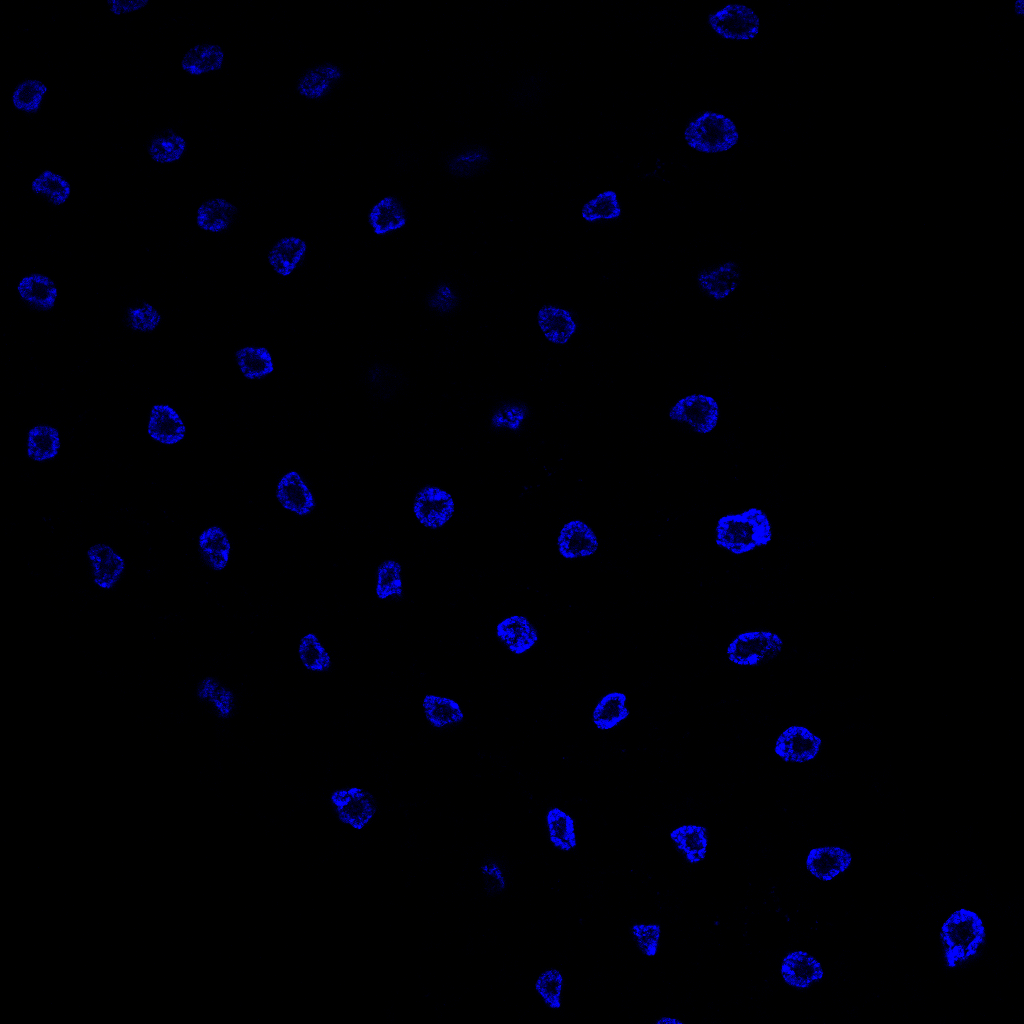
\includegraphics[width=\linewidth]{figs/img_nucleos1.png}

        (a) Canal utilizado para os núcleos.
    \end{minipage}
    \hfill
    \begin{minipage}{0.47\textwidth}
        \centering
        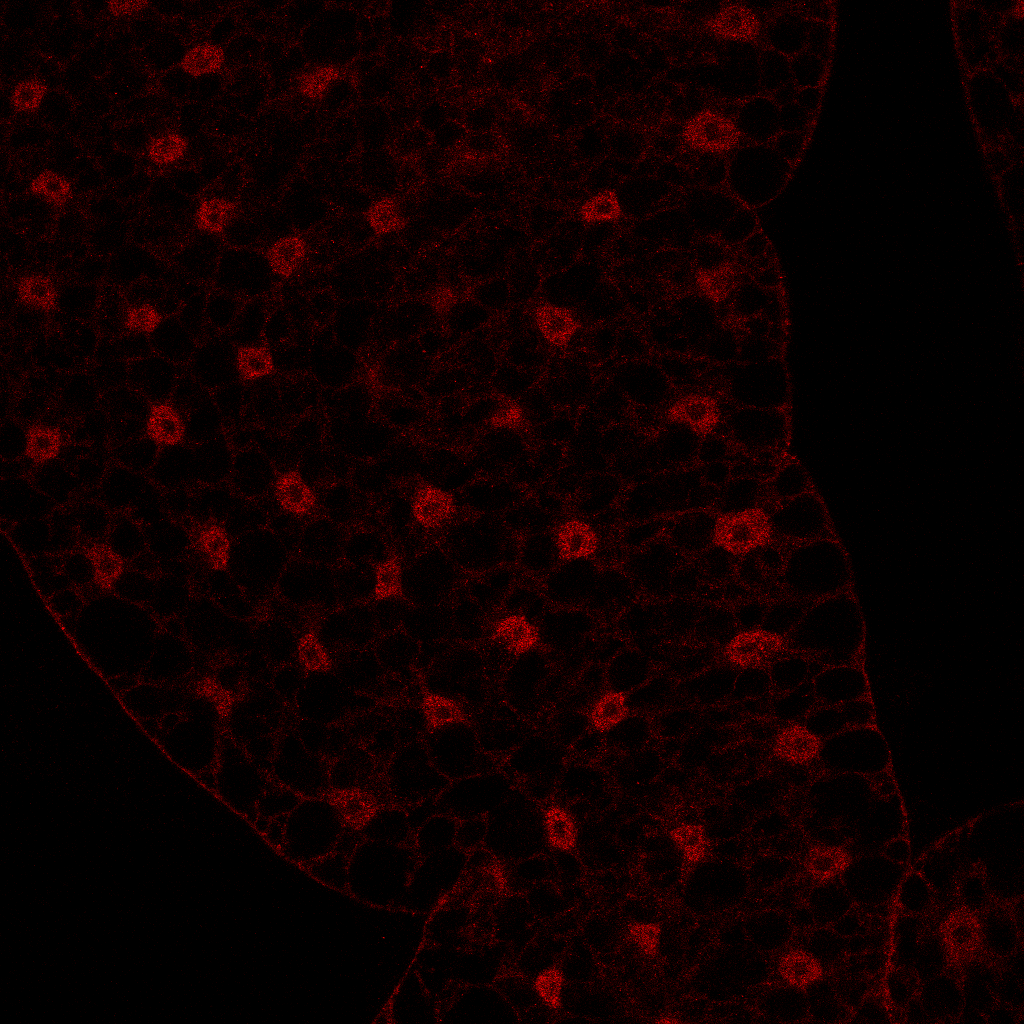
\includegraphics[width=\linewidth]{figs/img_proteina1.png}

        (b) Imagem correspondente de proteína.
    \end{minipage}
    \caption{Exemplo de par de imagens de fluorescência utilizado no pipeline.}
    \label{fig:par-fluorescencia}
    \fonte{Elaborado pelo autor (2026).}
\end{figure}

\section{Pipeline de processamento}
\label{sec:pipeline}

Cada par válido é submetido às etapas descritas a seguir.

\begin{enumerate}
    \item \textbf{Leitura e validação.} As imagens são lidas preservando a profundidade disponível. O algoritmo verifica existência, dimensionalidade, canais solicitados, dimensões espaciais compatíveis e chaves duplicadas.
    \item \textbf{Seleção de canal.} O canal 0 da imagem de núcleos é convertido para matriz de ponto flutuante e utilizado na segmentação. O canal 2 da imagem de proteína é preservado para a quantificação. A visualização normalizada não é usada nos cálculos.
    \item \textbf{Suavização e limiarização.} O sinal de núcleos é limitado ao intervalo de 8 bits, filtrado com Gaussiano de tamanho $5 \times 5$ e desvio-padrão 1,0; em seguida, recebe limiarização binária de Otsu.
    \item \textbf{Limpeza da máscara.} Uma abertura morfológica elíptica de tamanho $3 \times 3$ remove pontos isolados. Um fechamento elíptico de $5 \times 5$ reduz pequenas falhas internas.
    \item \textbf{Identificação de instâncias.} Componentes conectados com conectividade 8 são rotulados. Componentes com menos de 100 pixels são descartados e os identificadores restantes são remapeados para uma sequência contínua.
    \item \textbf{Medição por núcleo.} Para cada rótulo, os pixels internos são usados diretamente para calcular estatísticas do canal de proteína e atributos geométricos.
    \item \textbf{Saídas auditáveis.} O método salva máscara binária, sobreposição colorida, manifesto, configuração e tabelas CSV por núcleo e por amostra.
\end{enumerate}

A Tabela \ref{tab:parametros} sintetiza os parâmetros padrão. Eles são guardados em \texttt{configuracao.json}; portanto, uma alteração de parâmetro não fica implícita no resultado produzido.

\begin{table}[htb]
    \centering
    \caption{Parâmetros padrão do pipeline revisado.}
    \label{tab:parametros}
    \begin{tabular}{|p{0.40\textwidth}|p{0.18\textwidth}|p{0.29\textwidth}|}
        \hline
        \textbf{Parâmetro} & \textbf{Valor} & \textbf{Finalidade} \\
        \hline
        Canal de núcleos & 0 & Sinal empregado na segmentação. \\
        \hline
        Canal de proteína & 2 & Sinal empregado na quantificação. \\
        \hline
        Filtro Gaussiano & $5 \times 5$, $\sigma=1{,}0$ & Redução de ruído antes da limiarização. \\
        \hline
        Abertura / fechamento & $3 \times 3$ / $5 \times 5$ & Limpeza e preenchimento local da máscara. \\
        \hline
        Área mínima & 100 pixels & Remoção de componentes pequenos. \\
        \hline
    \end{tabular}
    \fonte{Elaborado pelo autor (2026).}
\end{table}

\section{Produtos da segmentação}

A Figura \ref{fig:produto-segmentacao} apresenta dois produtos do processamento de uma amostra. A máscara contém somente os núcleos preservados após a limpeza e o filtro de área. A sobreposição colorida é produzida exclusivamente para inspeção visual: ela permite conferir a correspondência espacial entre a imagem e os objetos segmentados, mas não é reutilizada para mensurar intensidade.

\begin{figure}[htb]
    \centering
    \begin{minipage}{0.32\textwidth}
        \centering
        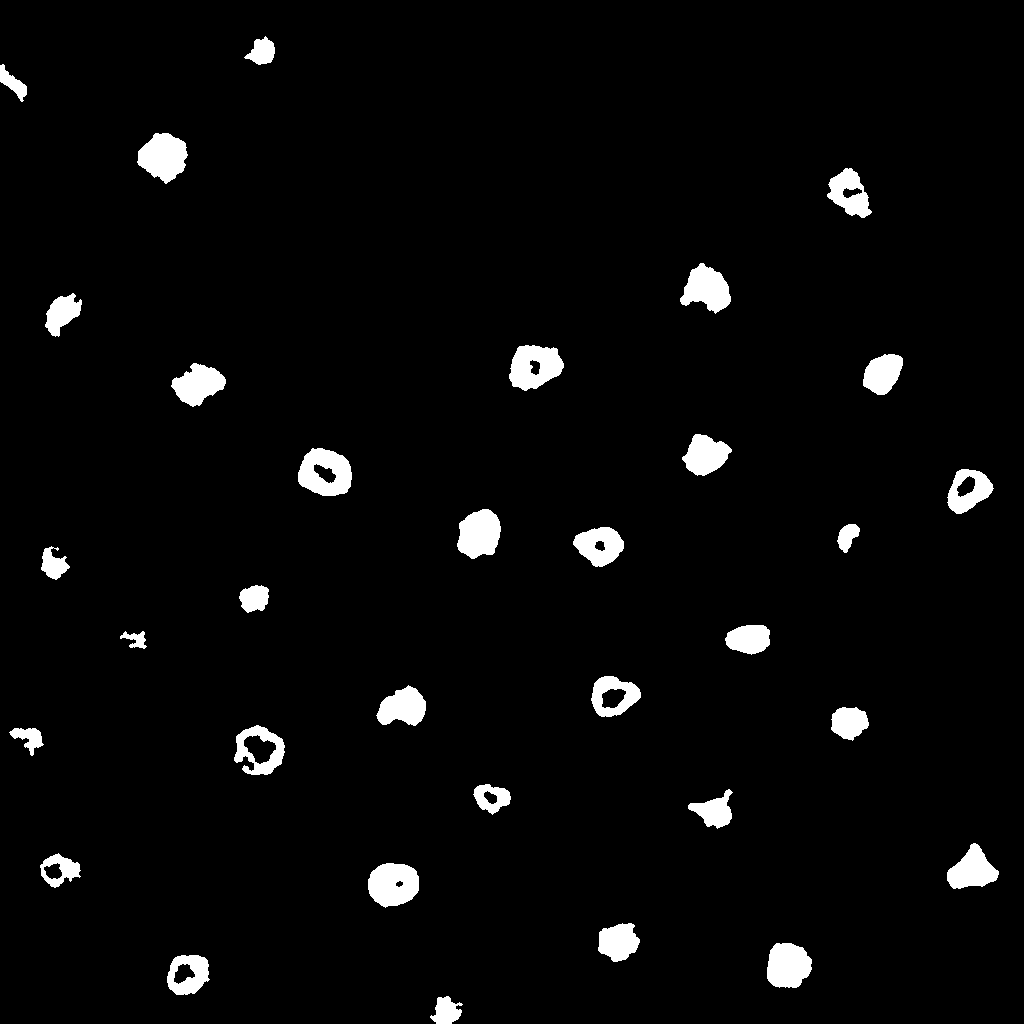
\includegraphics[width=\linewidth]{figs/mascara_exemplo.png}

        (a) Máscara binária.
    \end{minipage}
    \hfill
    \begin{minipage}{0.62\textwidth}
        \centering
        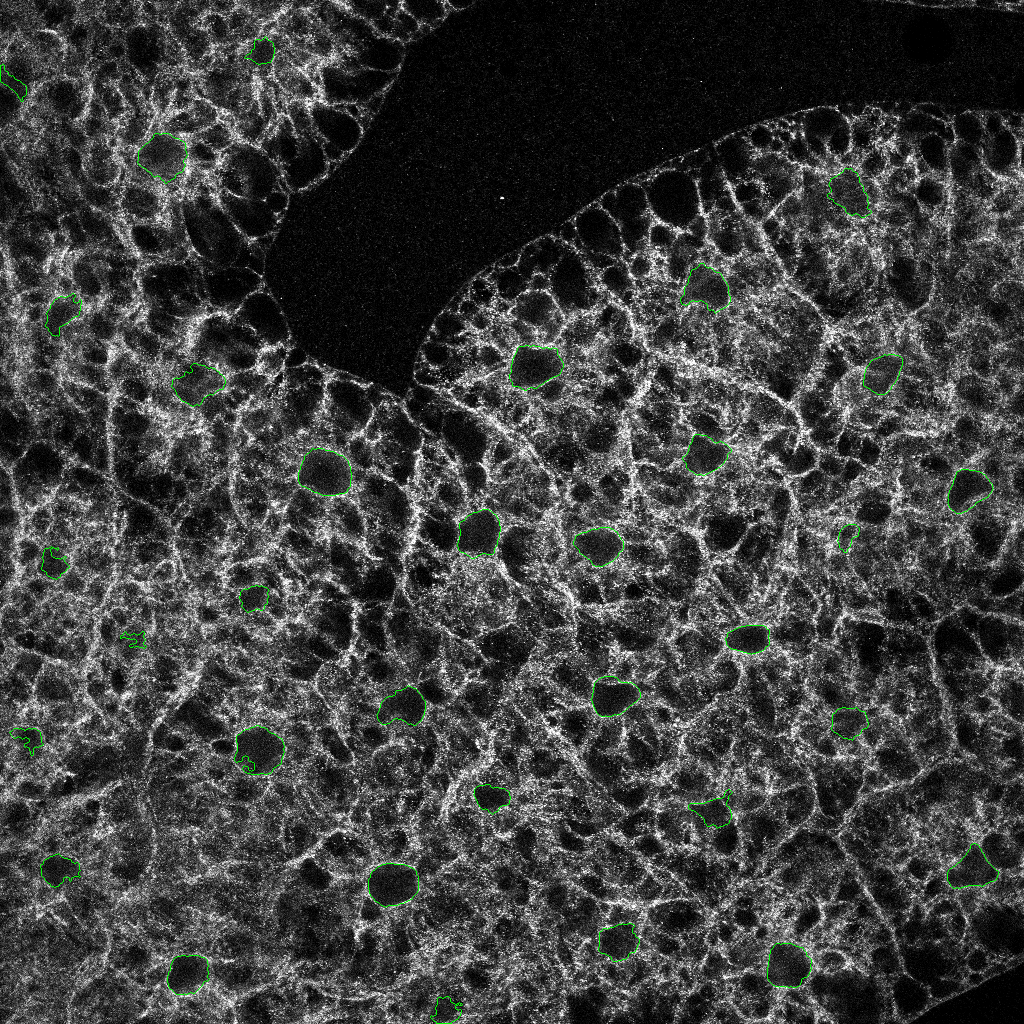
\includegraphics[width=\linewidth]{figs/sobreposicao_exemplo.png}

        (b) Sobreposição de controle de qualidade.
    \end{minipage}
    \caption{Exemplo de produtos gerados pelo pipeline revisado.}
    \label{fig:produto-segmentacao}
    \fonte{Elaborado pelo autor (2026).}
\end{figure}

\section{Medidas extraídas}

Cada núcleo recebe um identificador e um registro contendo área, área espacial quando o tamanho de pixel é informado, centroide, perímetro, raio e diâmetro equivalentes, eixos de elipse, excentricidade e circularidade. Para a proteína são calculadas média, mediana, desvio-padrão e intensidade integrada diretamente sobre os pixels internos. A média de uma amostra é a média das médias individuais dos núcleos; desse modo, imagens com maior número de objetos não dominam a estatística apenas por terem mais pixels.

O arquivo \texttt{resultados\_por\_nucleo.csv} é a saída analítica principal. O arquivo \texttt{resumo\_por\_amostra.csv} contém quantidade de núcleos, área total, limiar de Otsu e média por imagem. O manifesto e o arquivo de configuração completam a trilha de auditoria.

\section{Interface gráfica de revisão}

Além da execução em lote, foi construída uma aplicação web local composta por um cliente React com TypeScript e um servidor FastAPI. O servidor reutiliza as funções de leitura e segmentação do pipeline, executa trabalhos em um conjunto limitado de \textit{workers}, mantém sessões locais e armazena metadados e histórico em SQLite. O cliente permite selecionar as imagens, configurar canais e área mínima, visualizar as camadas de núcleo, proteína e máscara, selecionar objetos e exportar CSV ou JSON.

A edição de contorno recalcula apenas o núcleo modificado, e operações de ocultar, excluir e restaurar são registradas com revisão otimista. Caso duas operações partam de versões diferentes da mesma sessão, a API devolve conflito em vez de sobrescrever silenciosamente uma alteração. A interface também oferece desfazer e refazer. Nomes que indicam imagens derivadas, como máscaras ou sobreposições, geram aviso porque seus pixels podem não corresponder ao sinal bruto.

\section{Critérios de avaliação}

A avaliação operacional foi conduzida por três verificações: (i) execução dos testes de regressão do pipeline e dos testes da API e do cliente; (ii) inspeção visual das máscaras e sobreposições; e (iii) comparação das médias de intensidade por imagem com as saídas do algoritmo de referência em MATLAB. A comparação abrange 204 imagens distribuídas em oito conjuntos experimentais. Para cada imagem são comparadas a média de intensidade do algoritmo de referência e a média obtida pelo pipeline, além da contagem de núcleos. São reportados erro absoluto, erro relativo, proporção de imagens dentro de $\pm 10\%$ e correlação de Pearson. Como os dados disponibilizados para essa comparação são máscaras e imagens de borda derivadas, a análise verifica compatibilidade entre implementações; ela não substitui uma avaliação de acurácia de segmentação contra anotações manuais sobre os TIFFs brutos.

	% ----------------------------------------------------------
	% Experimentos e avaliação dos resultados
	% Obrigatório somente para TCC 2
	% ----------------------------------------------------------
	\chapter{Experimentos e análise dos resultados}
\label{cap:experimentos}

Este capítulo apresenta a avaliação do algoritmo proposto como alternativa ao algoritmo de referência desenvolvido em MATLAB por Breno. A análise principal utiliza os arquivos de comparação do conjunto \texttt{results13062022}, cujos resultados são organizados em \texttt{comparacao\_results13062022.csv} e \texttt{comparacao\_results13062022\_resumo.json}. O subconjunto local de 43 pares de TIFFs é utilizado no desenvolvimento e em testes de regressão, mas não representa a dimensão total da avaliação comparativa.

\section{Conjunto comparativo}

Foram comparadas 204 imagens, distribuídas em oito conjuntos experimentais. Para cada imagem, estão disponíveis uma máscara de núcleos, uma imagem de proteína com bordas de controle e um arquivo CSV com as medidas do algoritmo de referência. O conjunto reúne 13.740 núcleos no algoritmo de referência e 13.701 no algoritmo proposto. A diferença de contagem é pequena em escala global e é esperada quando duas implementações aplicam tratamentos de máscara independentes.

Os arquivos disponibilizados para a comparação são resultados derivados, e não os TIFFs brutos. Por essa razão, o pipeline proposto é aplicado sobre a máscara \texttt{ch00\_mask} e a imagem \texttt{ch02\_border}; pixels brancos pertencentes às bordas desenhadas são excluídos da medição de proteína. Essa decisão preserva o objetivo da avaliação: verificar se a implementação alternativa converge para as medidas já obtidas pelo algoritmo de referência. Ela não equivale a uma nova segmentação dos arquivos originais.

\section{Execução e controle de qualidade}

O processamento produz uma média de intensidade por imagem e a quantidade de núcleos associados. Os testes automatizados verificam o pareamento de arquivos, a seleção de canais e os fluxos da API. A inspeção visual das máscaras e sobreposições complementa a verificação numérica, permitindo identificar núcleos unidos, fragmentados ou indevidamente incluídos. A Figura \ref{fig:produto-segmentacao} ilustra os artefatos de controle de qualidade do pipeline.

\section{Convergência com o algoritmo de referência}

A Tabela \ref{tab:comparacao-metodos} sintetiza a avaliação. A média das médias de intensidade foi 30,944 no algoritmo de referência e 30,854 no algoritmo proposto. O viés médio foi de $-0{,}090$ unidade de intensidade e o erro absoluto relativo médio foi de 2,511\%. Em 202 das 204 imagens (99,02\%), a diferença absoluta ficou dentro de $\pm 10\%$. A correlação de Pearson entre as médias por imagem foi 0,9986.

\begin{table}[htb]
    \centering
    \caption{Comparação entre o algoritmo de referência em MATLAB e o algoritmo proposto.}
    \label{tab:comparacao-metodos}
    \begin{tabular}{|p{0.66\textwidth}|r|}
        \hline
        \textbf{Indicador} & \textbf{Valor} \\
        \hline
        Imagens comparadas & 204 \\
        \hline
        Conjuntos experimentais & 8 \\
        \hline
        Núcleos no algoritmo de referência & 13.740 \\
        \hline
        Núcleos no algoritmo proposto & 13.701 \\
        \hline
        Média das intensidades --- referência & 30,944 \\
        \hline
        Média das intensidades --- proposto & 30,854 \\
        \hline
        Erro absoluto médio & 0,920 \\
        \hline
        Erro relativo absoluto médio & 2,511\% \\
        \hline
        Imagens dentro de $\pm 10\%$ & 202 de 204 (99,02\%) \\
        \hline
        Correlação de Pearson & 0,9986 \\
        \hline
    \end{tabular}
    \fonte{Elaborado pelo autor (2026), a partir de \texttt{comparacao\_results13062022\_resumo.json}.}
\end{table}

Os resultados indicam forte convergência entre as implementações. A proporção de 99,02\% dentro da tolerância de 10\% supera o critério de convergência de 95\% adotado neste trabalho. A correlação de 0,9986 mostra que as variações de intensidade entre as imagens são preservadas de modo praticamente idêntico pelos dois algoritmos. Ao mesmo tempo, a análise da diferença por imagem evita que uma média global semelhante esconda divergências locais.

\section{Conjunto local de desenvolvimento}

O repositório contém 43 pares completos de TIFFs do conjunto de larvas desafiadas. Esse subconjunto foi usado para desenvolvimento, geração de imagens de controle de qualidade e testes de regressão do pipeline. A comparação adicional com as saídas correspondentes do algoritmo de referência apresentou correlação de Pearson de 0,9980 para as médias brutas de intensidade e erro relativo absoluto médio de 4,318\%. Esses resultados são consistentes com a avaliação ampliada, mas não devem ser confundidos com o total de imagens do experimento.

\section{Limitações e ameaças à validade}

A comparação de 204 imagens estabelece compatibilidade quantitativa com uma implementação de referência, mas não demonstra sozinha acurácia biológica absoluta. Primeiro, ela utiliza máscaras e imagens derivadas disponibilizadas pelo algoritmo de referência, e não os TIFFs brutos. Segundo, não foram utilizadas máscaras anotadas manualmente para calcular métricas de segmentação como \textit{Dice}, \textit{intersection over union}, \textit{precision} e \textit{recall}. Terceiro, o alinhamento espacial entre os canais deve ser validado caso se processem imagens brutas adquiridas ou exportadas separadamente.

Essas limitações não reduzem a evidência de convergência computacional apresentada, mas delimitam corretamente seu significado: o algoritmo proposto reproduz, com alta concordância, as medidas de intensidade do algoritmo de referência no conjunto disponível. A validação biológica em arquivos brutos e com anotações manuais permanece como etapa futura.

	
	% ---
	% Finaliza a parte no bookmark do PDF, para que se inicie o bookmark na raiz
	% ---
	\bookmarksetup{startatroot} 
	% ---
	
	% ---
	% Conclusão
	% Obrigatório somente para TCC 2
	% ---
	\chapter{Conclusão}
\label{cap:conclusao}

Este trabalho desenvolveu uma alternativa em Python ao algoritmo de referência implementado em MATLAB por Breno para a caracterização morfológica e a quantificação de proteína em imagens sagitais de \textit{Drosophila melanogaster}. A implementação final realiza pareamento de imagens por chave normalizada, seleção explícita de canais, segmentação de núcleos como instâncias individuais e medição da intensidade de proteína no interior dos objetos.

Na avaliação principal, foram comparadas 204 imagens de oito conjuntos experimentais. O algoritmo proposto alcançou correlação de Pearson de 0,9986 com as médias de intensidade do algoritmo de referência; 202 imagens, correspondentes a 99,02\% do total, apresentaram diferença absoluta de até 10\%, e o erro relativo absoluto médio foi de 2,511\%. Esses resultados confirmam a forte convergência entre as implementações e superam o critério de concordância de 95\% estabelecido para a comparação. O subconjunto local de 43 pares completos de TIFFs foi preservado para desenvolvimento, testes de regressão e controle de qualidade.

Também foi entregue uma interface gráfica local que permite inspecionar a imagem de núcleo, a proteína e a máscara, selecionar objetos, alterar o contorno de um núcleo, excluir ou restaurar registros e exportar os dados em CSV e JSON. O histórico de alterações e o controle de revisão preservam a rastreabilidade da revisão manual, aspecto importante quando a segmentação automática necessita da avaliação de especialistas.

\section{Limitações}

Os resultados comprovam a convergência computacional com a implementação de referência, mas não estabelecem validade biológica definitiva. A comparação foi realizada com máscaras e imagens de borda derivadas, pois os TIFFs brutos das 204 imagens não estavam disponíveis no conjunto comparativo. Também não foram utilizadas máscaras anotadas manualmente; portanto, não é possível quantificar acurácia de segmentação nem escolher parâmetros somente com base nas imagens resultantes. Núcleos encostados podem permanecer unidos e o alinhamento entre os canais deve ser verificado experimentalmente.

\section{Trabalhos futuros}

Como próximos passos, recomenda-se construir um conjunto de referência com máscaras manuais e avaliar a segmentação com métricas de sobreposição e de detecção de instâncias. Essa base permitirá calibrar área mínima, filtros e operações morfológicas, bem como avaliar a adoção de \textit{watershed} para núcleos aglomerados. Também será possível comparar de forma justa o pipeline clássico a métodos de aprendizado profundo, como U-Net \cite{Ronneberger2015} e StarDist \cite{Schmidt2018}.

Outra extensão consiste em incorporar registro espacial entre canais, controles de aquisição e procedimentos de normalização que sustentem comparações quantitativas entre experimentos. A interface pode evoluir com anotações assistidas, visualização de distribuições e importação de metadados experimentais. Dessa forma, o trabalho estabelece uma base computacional auditável para futuras análises biológicas, sem antecipar conclusões que dependem da validação experimental.
	
	% ----------------------------------------------------------
	% ELEMENTOS PÓS-TEXTUAIS
	% ----------------------------------------------------------
	\postextual
	
	% ----------------------------------------------------------
	% Referências bibliográficas
	% ----------------------------------------------------------
	\bibliography{bib/modelo-referencias,bib/ref}

	
	% ----------------------------------------------------------
	% Glossário - opcional
	% ----------------------------------------------------------
	%
	%\glossary
	
	% ----------------------------------------------------------
	% Apêndices  - opcional
	% ----------------------------------------------------------
	% ---
	% Inicia os apêndices
	% ---
	\begin{apendicesenv}
		% Imprime uma página indicando o início dos apêndices
		\partapendices
		% ----------------------------------------------------------
		% Incluir Apêndice
		% ----------------------------------------------------------
		% Capitulo com exemplos de comandos inseridos de arquivo externo 
		% ----------------------------------------------------------
		\chapter{Reprodução do processamento}
\label{ap:reprodutibilidade}

O código-fonte, as imagens de controle de qualidade e os arquivos CSV gerados pelo pipeline acompanham este trabalho. A execução abaixo deve ser realizada a partir da raiz do repositório, após a instalação das dependências declaradas em \texttt{requirements.txt}.

\begin{verbatim}
python -m pip install -r requirements.txt
python pipeline_melhorado.py --verbose
python comparar_resultados.py
python -m unittest -v test_pipeline_melhorado.py
python -m pytest backend/tests -q
\end{verbatim}

Para utilizar a interface local, inicia-se a API em um terminal e o cliente web em outro:

\begin{verbatim}
python -m uvicorn backend.app.main:app --reload --port 8000
cd frontend
npm install
npm run dev
\end{verbatim}

O processamento gera o manifesto de pares, a tabela por núcleo, o resumo por amostra, o arquivo de configuração e as imagens de máscara e sobreposição. Esses artefatos permitem auditar parâmetros, conferir a associação entre os canais e repetir a análise com o mesmo conjunto de dados.

		
	\end{apendicesenv}
	% ---
	
	% ----------------------------------------------------------
	% Anexos  - opcional
	% ----------------------------------------------------------
	% ---
	% Inicia os anexos
	% ---
	\iffalse % Não há anexos neste trabalho.
		% Imprime uma página indicando o início dos anexos
		\partanexos
		% ---
		% Incluir Anexo
		% ---
		% Sem anexos no trabalho final.
		
	\fi
	
	
\end{document}
